\section{Wednesday for MAT3006}\index{Monday_lecture}
\subsection{Remarks on Baire Category Theorem}
\begin{theorem}[Baire Category Theorem]
If $(X,d)$ is complete, and $E_i\subseteq X$ is nowhere dense for $i\in\mathbb{N}$, then
\[
\bigcup_{i=1}^\infty\overline{E}_i
\]
contains no open balls.
\end{theorem}


\begin{definition}
Let $(X,d)$ be a complete metric space. 
\begin{enumerate}
\item
We say $S\subseteq X$ is \emph{meager} if 
\[
S=\bigcup_{i=1}^\infty E_i,\ \quad\text{$E_i$ is nowhere dense}
\]
In this case we say $S$ is of \emph{first category}.
\item
$S'\subseteq X$ is \emph{comeager} if
\[
S'=X\setminus S, \ \quad\text{where $S$ is meager}
\]
\end{enumerate}
\end{definition}
For example, $\mathbb{Q} = \cup_{x\in\mathbb{Q}}\{x\}$ is megre; $\mathbb{R}\setminus\mathbb{Q}$ is comeager.
\begin{remark}
\begin{enumerate}
\item
By the Baire Category Theorem, $\cup_{i=1}^n\bar{E}_i$ contains no open balls, i.e.,
\[
S:=\cup_{i=1}^\infty{E}_i\subseteq \cup_{i=1}^\infty\bar{E}_i
\]
contains no open balls.
\item
$S'$ is comeager implies $S'$ is dense in $X$: for $\forall x\in X$, $B_{1/n}(x)\cap S'$ is non-empty, since otherwise $X\setminus S'$ contains a open ball, which is a contradiction. Therefore, $x\in\overline{S'}$.
\end{enumerate}
\end{remark}



\begin{proposition}
If a set $S$ is meager, it cannot be comeager and vice versa.
\end{proposition}

\begin{proof}
Suppose on contrary that $S$ is meager and comeager, then
\begin{align*}
S&=\bigcup_{i=1}^\infty E_i,\ \quad\text{$E_i$ is nowhere dense}\\
X\setminus S&=\bigcup_{j=1}^\infty F_j, \ \quad\text{$F_j$ is nowhere dense}
\end{align*}
Therefore, 
\[
X = \bigcup_{i=1}^\infty E_i\cup\bigcup_{j=1}^\infty F_j
\]
is a countable union of nowhere desne sets. By applying Baire Category Theorem, $X$ has no open balls, which is a contradiction.
\end{proof}

\begin{remark}
We say $S\subseteq X$ is of \emph{first category} if $S$ is meager.
Any subset that is not of first category is of \emph{second category}.
Therefore, comeager implies second category.

We illustrate the relationship above in the figure below:
\begin{figure}[H]
\centering
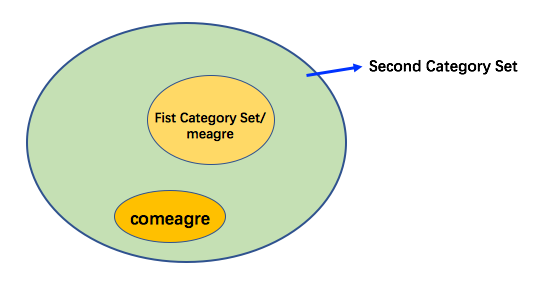
\includegraphics[width=0.9\textwidth]{week5/p_4}
\end{figure}
Note that there are subsets that are \emph{neither meager nor co-meager}.
\end{remark}


\begin{example}
\begin{enumerate}
\item
Here is another proof of $[0,1]$ is un-countable: Suppose on the contrary that $[0,1]$ is countable, then we imply 
\[
[0,1] = \bigcup_{n\in\mathbb{N}}\{x_n\},\quad\text{for some $x_n$.}
\]
Applying Baire Category Theorem (since $[0,1]$ is complete), $[0,1] = \cup_{n\in\mathbb{N}}\{x_n\}$ contains no open balls. However, the open ball $(0.5,0.7)\subseteq[0,1]$, which is a contradiction.
\item
The set $X:=\mathcal{C}[a,b]$ is complete.
\begin{enumerate}
\item
The set of all nowhere differentiable functions is \emph{of 2nd Category} in $\mathcal{C}[a,b]$. (Check Theorem~(4.1) in MAT2006)
Actually, the set of all nowhere differentiable functions is \emph{comeager}. The proof for this statement is omitted.
\item
Due to the relationship 
\[
\mathcal{P}[a,b]\subseteq\mathcal{C}^\infty[a,b]\subseteq\{f:[a,b]\to\mathbb{R}\mid \text{$f$ is differentiable somewhere}\}
\]
and that the last subset is meager, we imply $\mathcal{P}[a,b]$ and $\mathcal{C}^\infty[a,b]$ is meager.
\end{enumerate}
\end{enumerate}
\end{example}

\subsection{Compact subsets of $\mathcal{C}[a,b]$}

Recall that for metrice spaces, the compactness implies closed and bounded, but in general the converse does not hold. We will study extra conditions to make subsets of $\mathcal{C}[a,b]$ compact.
\begin{definition}[(Uniformly) Bounded]
The subset $S$ in metric space $(\mathcal{C}[a,b],d_\infty)$ is \emph{(uniformly) bounded} if there exists $M>0$ such that
\[
\sup_{f\in S}\|f\|_\infty = M
\]
\end{definition}
In next class, we will show that $K\subseteq\mathcal{C}[a,b]$ is compact if and only if 
$K$ is closed,(uniformly) bounded, and equi-continuous.













